\documentclass[12pt,reqno]{amsart}
\usepackage{../handout, ../customcommands}
\usepackage{caption}

\hdr{MAT 240}{\S3.6 Conditional distributions, part 1}

\begin{document}

\textbf{Suggested problems:} 2-4, 6-10

\bigskip
\hrule

\bigskip
\prob Insurance companies keep track of how likely various cars are to be stolen. Suppose that a company in a particular area computes the joint distribution of car brands and the indicator of whether the car will be stolen during a particular year that appears in the table below.

\medskip
\begin{center}
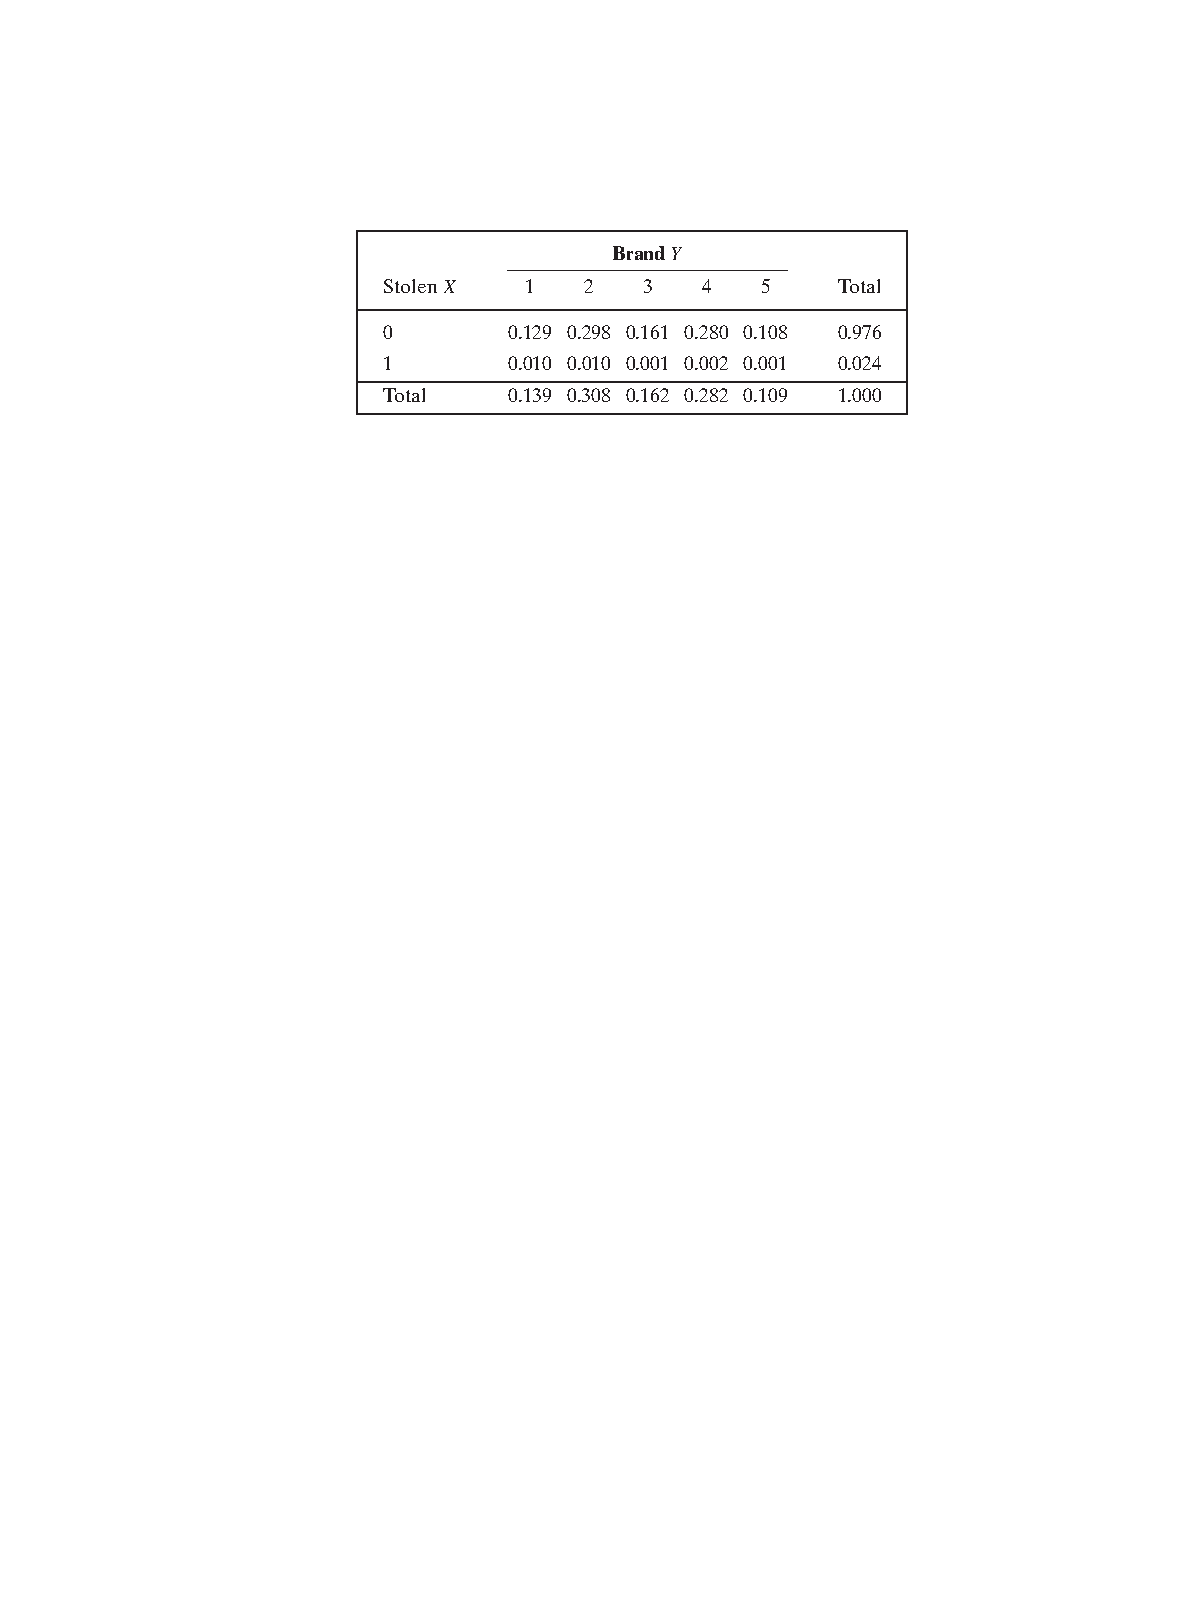
\includegraphics[scale=1]{1.pdf}
\end{center}

Compute the conditional probability function $g_{X\mid Y}(x\mid y)$. Which brand of car is most likely to be stolen?

\vfill
\prob A manufacturing process consists of two stages. The first stage takes $Y$ minutes, and the whole process takes $X$ minutes (which includes the first $Y$ minutes). Suppose that $X$ and $Y$ have a joint continuous distribution with probability density function
\[
	f(x,y) = \begin{cases}
	e^{-x} & : 0 \leq y \leq x, \\
	0 & : \text{else}.
	\end{cases}	
\]
Compute the conditional probability density function $g_{X\mid Y}(x\mid y)$.

\vfill
\end{document}